{
{\sffamily Vi bør introducere problematikken ved billedbehandling her.
Hvorfor er det at computeren ikke bare kan ``se'' ligesom mennesket.
Hvordan opfatter computeren et billede. Giv en latterlig analogi, f.eks.
en blind mand der bliver fortalt hvilken farve hver kvadratcentimeter
har på et maleri og at han ud fra de oplysninger skal afgøre hvordan
billedet tager sig ud.

Vi bør i denne sammenhæng også komme ind på at billedbehandling, især
ikke det givne problem, er veldefineret. Det er nok en afart af det
ovenstående, men det bør understreges.
}

\subsection{Opdeling af billeder}
\textsf{
Mange af de metoder, vi bruger til at udregne, det gyldne snits position
eller størrelsen af en margin, udregnes med brøker. Hvorimod et billede
opbygges af pixels. Dette gør, at vi bliver nødt til at tage
approksimationer af udregningerne. Vi vil også kommer ind på nogle af de
fejl som kan opstå i tilblivelse af maleriet}

\subsection{Inddeling af billede efter snit}
Vi vil i dette afsnit give nogle definitioner på hvordan et billedet er
bygget op, samt hvilke afrundings fejl der kan opstår ved denne
opbygning. For at få nogle faste definitioner på hvordan et billedet ser
ud samt hvad et snit er, har vi stillet de her to definitioner op.

\begin{definition}
	I et billede betegnes \textbf{højden og bredden} som hhv. $H$ og
	$B$, som illustreres i figur \ref{cut}.
\end{definition}

\begin{definition}
	Et \textbf{snit} er en lige vertikale eller horisont linje, som
	strækker sig fra kant til kant.
\end{definition}

\begin{figure}[h]
	\begin{center}
		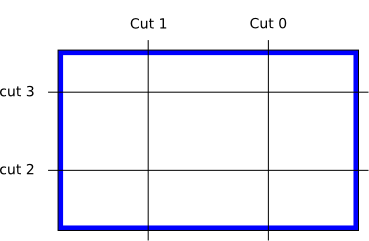
\includegraphics[scale=0.42,angle=0]{afsnit/vores_implementation/billeder/naiv_algoritme/Cut}
	\end{center}
	\caption[]{Billedets højde og bredde betegnes hvv. H og B. De 4 snit er navngivet.}
	\label{cut}
\end{figure}

End til vider har vi kun arbejder med det gyldne snit, men andre snit i
billedet kan godt optræde, derfor indføre vi en nu betegnelse
snitratio.

\begin{definition}
	En \textbf{snitratio} er en procents sats, som ganget på $B$ eller
	$H$, finde placeringen af et snit i billedet.
\end{definition}

Det vil sige at hvis en snitration er på $0.2$. Et billedet har $B$ på
4000 vil et snit befinde sig i pixel $4000*0.2 = 800$ fra højre side af
billedet, det samme antal pixel fra venstre side vil også være et snit.
Samme metode kan bruges på $H$ for at få 2 snit mere. 

\begin{definition}
	For vær snitration er der fire snit, to i det vertikale plan og to i
	det horisontale plan, som er illustreret på maleri \ref{lenasnit2},
	med røde streger. Med mindre snitration er 0.5, så er der kun 2 snit.
\end{definition}

Hvis snitratioen er $0.5$ kommer snittene til at ligge over på hinanden,
og derved vil snitratioen kun have 2 snit, de 2 snit Id, samt snitenes
plascring kan ses i figur \ref{2Cut}.

\begin{figure}[h]
	\begin{center}
		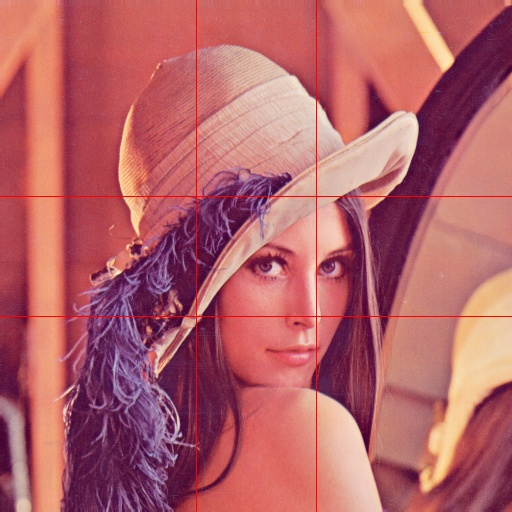
\includegraphics[scale=0.42,angle=0]{afsnit/vores_implementation/billeder/naiv_algoritme/Lenagolden}
	\end{center}
	\caption[]{Billedet som har indtegnet de fire gyldne snit}
	\label{lenasnit2}
\end{figure}

De 4 snit tildeles hvert deres Id, "snit 0,1,2 og 3" så vi kan kende
forskel på de individuelde snit, Id'erne placering kan ses i figur
\ref{cut}. Vi vil i resten af rapporten kalde snittene efter deres Id.

\begin{definition}
	Vær snit af vær snitratio, har et fast \textbf{Id}, "Snit 0,1,2 og 3", som kan ses i figur \ref{cut}, hvor vært snit er indtegnet, samt deres Id som label. 
\end{definition}

\begin{figure}[h]
	\begin{center}
		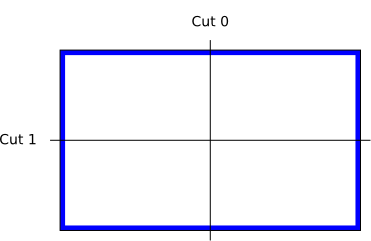
\includegraphics[scale=0.42,angle=0]{afsnit/vores_implementation/billeder/naiv_algoritme/2Cut}
	\end{center}
	\caption[]{Billedet skæres her kun af 2 snit}
	\label{2Cut}
\end{figure}

\subsection{Acceptabel afvigelse}
\begin{comment}"""
Som beskravet i afsnit \ref{mange_tal}, udregnes det gyldne snit med mange decimaler. Selv den beste kunstner har et maksimum på hvor præcis han kan male, om det er hans øjne der sætter grandsen eller størrelsen på han pensler eller om han bare ikke maler særlige præcis, så kan han aldrig malle så præcis som vi kan udregne det gyldne snit til. Derfor sætter vi en afvigelse på $0.5 \%$, som maleren vi sat en 
\end{comment}
\note{Nogle referanse}Som beskrevet i afsnit \ref{mange_tal}, udregnes
det gyldne snit med mange decimaler. En kunstner, hvor god han end er,
har ingen chance for at male så præcist at man kan sige at strøget
ligger nøjagtigt oven på snittet selv om hans intentioner er at ramme
snittet. Vi kommer derfor til at have en vis uprecis hed på de data vi
få fra billedet selv. Vi starter med at se på alle de ting, som kan
skabe en usikkerhed fra malerens side. Man kan gå ud fra at den
procentvise afvigelse ikke er særlig stor, da vi ikke har bestræbelser
på at arbejde på abstrakt malerier, dog har vi sat den procentvise
afvigelse til 0.5 \%. Det vil sige at en maler med et lærred på 100
cm, maksimalt vil male $0.5$ cm forkert.

Når maleren vælger en ramme og et lærred, har vi igen problematikken,
selv om maleren spicifikt gå efter at bygge maleriet op efter det gyldne
snit, kan snittets placering i maleriet have forskubbet sig, ved dårlige
valg at ramme eller lærred. Derfor sætter vi den afvigelse til $1\%$. Da
vi igen mener at dette er den maksimale afvigelse, der kan opstå.

Når maleren maler en region i et maleri, forekommerer der normalt en
lille kant rundt om objektet, et omrids. Dette omrids kan vores
algoritmer ikke tage højde for, og vi må derfor modregne omridset, så vi
er sikre på at vi ser på regionen og ikke dens omrids. Da et omrids ikke
er særligt stort, har vi sat denne procentsats til $0.5\%$. 

Alt i alt giver det en afvigelse på vores aktuelle udtrækning af data
fra malerierne på $2\%$ det vil sige at finder vi en region, som ligger
på pixel 200, i et billedet, der er $500$ cm bredt, befinder den sig
faktisk i intervallet [190,210]. Måden hvorpå vi tager højde for den
forskel, er ved hjælp af marginer, som nævnt i afsnit
\ref{section_naiv}.


\subsection{Heltal i det gyldne snit}
Nå vi udregner hvor et snit for et billedet med $H = 4000$,
approksimerer vi antal pixels ved at afrunde resultatet $2472.13595
\approx 2472$, se udregning \ref{afrundning}. Det betyder at vi mister
0.13595 pixels i præction, hvilket svarer til en misvisning af punktet
på 0.00339875 $\%$ i forholdt til $B$ på billedet. Se udregning
\ref{afrundning2}.

\begin{equation}
	4000 \cdot \varPhi = 4000(\sqrt{5}-1)/2 = 2472.13595 \approx 2472 \label{afrundning}
\end{equation}

\begin{equation}
	0.13595/4000 \cdot 100 = 0.00339875 \label{afrundning2}
\end{equation}

Det er en meget lille del af selve billedet og skulle ikke give nogle
misvisninger i forhold til udregningen. For at gøre det lidt mere
generelt, sætter vi trunkeringsfejlen til $0.5$, da det er den maksimale
afrundingsfacktor som kan forekomme. Hvis billedet har en størrelse på
500 pixels, hvilket er det mindste billedet vi har, giver dette en fejlmargin
på $0.1 \%$. Dette tal bliver adderet til fejlsatsen ovenfor, og giver
en samlet afvigelse på $2.1\%$.



\subsection{Heltal ved udregning af Margin}
Når vi har 2 forskellige snitratioer, f.eks. $\varPhi$ og $\frac{2}{3}$,
som ligger meget tæt på hinanden, og vi gerne vil sammenligne hvilken
regioner der ligger i snitratioernens snit, er det vigtigt at margin for
vært af de 2 snitratioers snit ikke krydser hinanden. 

Hvis margin krydser. Vil det indebære, at den samme region bliver fundet
af begge snit. Dette vil give et skævt billedet af forskellen på de to.
Derfor må vi sørge for at marginerne ikke krydser. Hvis $x$ betegner
antal pixels i $B$ eller $H$, og vi vil se på, hvor mange pixels, der er
mellem snitratio $\frac{2}{3}$ og $\varPhi$, multiplicerer vi $x$ med de
to snitratioen for at finde deres placering. Derefter subtraheres vi et
af de snit som befinder sig tetest på hinanden i vær snitratio med
hinanden.


\begin{eqnarray}
	\frac{x2}{3} - \frac{x2}{\sqrt{5}+1} & = & x(\frac{2}{3} - \frac{2}{\sqrt{5} + 1}) \nonumber \\
	& = & x(0.666667-0.618034) \\ \nonumber
	& = & x(0.048633)
\end{eqnarray}

Vi har nu fundet antal pixel mellem de to snit. Vi vil gerne undgå at
de to marginer krydser hinanden, så vi dividere antal pixel mellem de to snit med to og afrunder værdien.

\begin{equation}
	\left\lfloor \frac{0.048633x}{2}\right\rfloor = \left\lfloor0.024316x \right\rfloor
	\label{marginstoerlse}
\end{equation}

Den minimale procentvise størrelse, margin må have, når vi
sammenligner det gyldne snit og $\frac{2}{3}$, er altså $2.4316$ Det
betyder også, at vi ikke må sammenligne snit som ligger særlig meget
tætter på hinanden, da $2.1\%$ er den minimale procent margin som vi må
have. For at vise, hvor stor marginen egentlige kan være, bruger vi formel \ref{marginstoerlse} på to billeder, et, som svarer til vores mindste billede, på
500 pixels, og et, som svarer til vores største billede, på 4000 pixels. Ved
500 pixels bliver resultatet.

\begin{definition}
	Margins størrelse i et snit, må ikke overstige $2.4316 \%$, af det respektive maleri $B$ eller $H$.
	\label{margin_max}
\end{definition}

\begin{definition}
	Margins størrelse i et snit, må ikke kommer under $2.1 \%$, af det respektice maleri $B$ eller $H$.
	\label{margin_min}
\end{definition}

\note{Er det denne måde det skal stilles op?}
\begin{equation}
	 \lfloor 500(0.024316)\rfloor = 12
\end{equation}

Det er en fin margin, da vores fejl på udregningerne ligger på 2.1 \%,
som svarer til $\lceil 500*0.021 \rceil = 11$ pixels. Der er 1 pixel fra vores
margin.

Ved 4000 pixels giver det.

\begin{equation}
	 \left\lfloor 4000(0.024316)\right\rfloor = 97
\end{equation}

Som også er god nok, da $4000*0.021 = 84$ pixels.
% vim: set tw=72 spell spelllang=da:


\subsection{Opbevaring af billeder}
{
En central del af den automatiserede analyse af malerier er den database
hvor vi opbevarer metadata og resultater. Vi vil til at starte med kun
koncentrere os om maleriernes metadata og først i afsnit
\ref{section_results} se på hvordan vi i databasen opbevarer resultater.
Dette gøres fordi vi endnu ikke har været inde over hvilke resultater
der kunne være interessante at gemme.

Vi bruger SQLite til selve databasen, hovedsageligt fordi der ikke kræves
nogen videre konfiguration af en sådan database. Den underliggende
database er dog underordnet, da vi bruger Python-pakken \emph{SQLObject}
som giver et abstraktionslag til en bred vifte af databaser. Vi opretter
blot de tabeller vi ønsker at have i databasen som klasser gennem
Python. Ligeledes får vi en sådan klasse tilbage når der laves
forespørgsler til databasen. Da \emph{SQLObject} klarer al kommunikation
med databasen er det derfor muligt at skifte den underliggende database
ud hvis man ønsker det. Vi ser dog ikke nogen grund til at bruge en
anden foreløbig, da SQLite opfylder vores behov. Endvidere har SQLite
den umiddelbare fordel at selve databasen lægges i en fil i filsystemet.
Det er derfor en let sag at tage sikkerhedskopier af databasen uden alt
for meget besvær.

Vores korpus består af billeder hentet fra hjemmesiden \cite{wgahu} som
indeholder europæiske kunstartikler fra år 1001 -- 1900. I
kunstartiklerne, hvor det samlede antal er omkring 23.000, indgår
møbler, skulpturer, mosaikker og malerier, hvor sidstnævnte vil være
vores fokus. Fra \cite{wgahu} tilbydes en kommasepareret fil over hele
deres database som vi har brugt til at populere vores egen database med.
Der gives mange oplysninger om den enkelte artikel samt dennes kunstner.
Vi har konstrueret en parser som trækker disse informationer ud fra
filen og lægger dem ind i tabellerne \ref{artistTable0} og
\ref{paintingTable0} i databasen. Da vi primært vil beskæftige os med
malerier vil vi nu blot omtale kunstartikler som malerier.

\begin{table}[!h]
    \centering
    \begin{tabular}{|l||c|c|c|c|c|c|}
        \hline
        \bf{artist} \hspace{0.5cm} & \underline{artistId} & name & born & died & school & timeline \\\hline
    \end{tabular}
    \caption{Databasetabel for kunstner}
    \label{artistTable0}
\end{table}

\begin{table}[!h]
    \centering
    \begin{tabular}{|l||c|c|c|c|c|c}
        \hline
        \bf{painting} \hspace{0.5cm} & \underline{paintingId} & artistId & title & date & paint & $\cdots$ \\\hline
    \end{tabular}\\ \vspace{0.2cm}\hspace{1.2cm}
    \begin{tabular}{c|c|c|c|c|c|c}
        \hline
        $\cdots$ & material & location & url & form & type & $\cdots$ \\\hline
    \end{tabular}\\ \vspace{0.2cm}\hspace{1.4cm}
    \begin{tabular}{c|c|c|c|c|c|}
        \hline
        $\cdots$ & realHeight & realWidth & height & width & filepath \\\hline
    \end{tabular}
    \caption{Databasetabel for malerier}
    \label{paintingTable0}
\end{table}

Ovenstående databaseskema lægger vægt på at vi let kan forespørge
databasen ved en lang række parametre, såsom et maleris fysiske
størrelse eller kunstneres fødselsår. Vi har, at en der til en kunstner
kan være tilknyttet en række malerier og at der til et givet maleri kun
kan være én kunstner. I den kommaseparerede fil fra \cite{wgahu} er
malerier opstillet efter kunstneren, hvilket gør det let først at
oprette denne i databasen og derefter oprette de efterfølgende malerier
tilknyttet denne kunstner.

Den konstruerede parser til den kommaseparerede fil er dog ret grov, da
folkene bag \cite{wgahu} ikke har lagt meget vægt på at være konsistente
i deres formulering af en kunstners fødsels- og dødsår eller en
genstands dimensioner. En følge deraf er, at nogle kunstnere, hvor
\cite{wgahu} ikke har en klar indikation af dennes levealder, ikke bliver
registreret i databasen. Vi kan dog stadig slå kunstneren op ved at
bruge feltet ``timeline'' i tabel \ref{artistTable0} som angiver hvilken
periode kunstneren tilhører. Vi har i enkelte tilfælde set os nødsaget
til at rette i den kommaseparerede fil i tilfælde hvor der er blevet
indsat tegn der helt umuliggør korrekt parsing, såsom ekstra komma
eller semikolon.

Givet den kommaseparerede fil fra \cite{wgahu} er det en smal sag at
konstruere en crawler som henter alle billederne fra hjemmesiden ned. I
filen gives nemlig en henvisning til hvor man kan finde et billede af
genstanden på deres side. Billederne hentes ned og gemmes på filsystemet
i samme mappestruktur som der bruges på \cite{wgahu}. Her indeles
filerne i mapper navngivet efter deres kunstner. Kunstnerenes mapper
inddeles efter forbogstav. På denne måde undgås problemet at to billeder
kan have det samme filnavn. Filstrukturen er grafisk illustreret i figur
\ref{mappestruktur}. Vi gemmer da blot stien til en fil på filsystemet i
databasen.

% Mappestruktur
\begin{figure}[!h]
    \centering
$
\xymatrix{
 &  &   & \ar @{-} [d] \textrm{/res}  &                                                     \\
 &  &   & \ar @{-} [d] \textrm{/wga.hu}  &                                                  \\
 &  &   & \ar @{-} [dl] \ar @{-} [d] \ar @{--} [dr] \textrm{/art} &                         \\
 &  & \ar @{-} [dl] \ar @{-} [d] \ar @{--} [dr] \textrm{/a} & \textrm{/b} & \cdots          \\
 & \ar @{-} [dl] \ar @{-} [d] \textrm{/aachen} & \ar @{--} [d] \textrm{/abadia} & \cdots    \\
\textrm{allegory.jpg} & \textrm{bacchus.jpg} & \cdots &   &
}
$
    \caption{Mappestruktur til filer fra
        \href{http://www.wga.hu}{http://www.wga.hu}}
    \label{mappestruktur}
\end{figure}

Som tidligere nævnt så vil vi i afsnit \ref{section_results} bygge
videre på databasen når vi skal gemme resultater fra en automatiseret
analyse. Indtil videre vil den beskrevne database blot bruges til at
trække filnavne på malerier ud til videre analyse.

}
% vim: set tw=72 spell spelllang=da:


\subsection{Floodfill}
% Denne fil er inkluderet i udtraekning_af_regioner.tex
{

Floodfill finder de områder i et billede, hvis farve ligger inden for en
vis afvigelse af den originale farve. Der vælges en pixel i billedet,
som har en farve angivet ved en RGB-værdi. Ud fra denne pixel findes de
fire tilstødende pixels i lodret og vandret bane, som vist i figur
\ref{floodfill1}.

\begin{figure}[!h]
    \begin{center}
        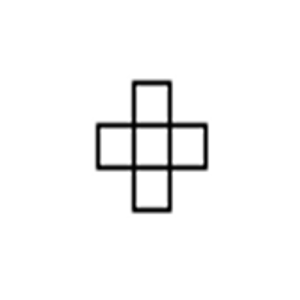
\includegraphics[scale=0.42,angle=0]{afsnit/vores_implementation/billeder/flood_fill/floodfill1}
    \end{center}
    \caption[]{Måden hvorpå floodfill arbejder med pixels i billedet.}
    \label{floodfill1}
\end{figure}

\subsubsection{Metode}
De følgende 3 skridt beskriver, hvordan floodfillmetoden virker i et
billede.

\begin{enumerate}
    \item Algoritmen starter med at markere den midterste pixel (vores
        startpixel) med et rødt flag, som angiver, at denne pixel bliver
        farvet. Nabopixels får et blåt flag, som angiver, at de skal
        kontrolleres for, om deres farve er inden for afvigelsen. Blå
        flag sættes kun, hvis en pixel ikke har noget flag i forvejen.
        Se figur \ref{floodfill2}.
    \item Hver pixel med et blåt flag kontrolleres for, om deres farve
        ligger indenfor afvigelsen. Hvis farven er inden for afvigelsen,
        bliver denne pixel sat i en liste og markeret med et grønt flag
        og et tal. Se figur \ref{floodfill3}.
    \item En pixel med grønt flag tages ud af listen og bliver sat til
        den nye startpixel. Skridt $1$ og $2$ bliver gentaget, til der
        ikke er flere grønne flag. Se figur \ref{floodfill4}.
\end{enumerate}

\begin{figure}[!h]
    \begin{center}
        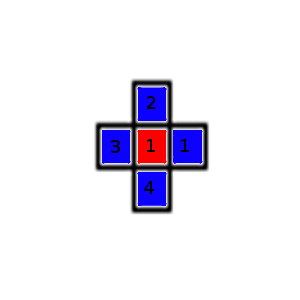
\includegraphics[scale=0.42,angle=0]{afsnit/vores_implementation/billeder/flood_fill/floodfill2}
    \end{center}
    \caption[]{Pixels efter første skridt i algoritmen. Den røde pixel
    er vores startpixel. Pixels, markeret med blåt, skal kontrolleres for
    deres farve. Numrene angiver rækkefølgen hvori de bliver gennemgået.}
    \label{floodfill2}
\end{figure}

\begin{figure}[!h]
    \begin{center}
        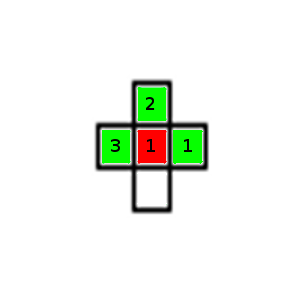
\includegraphics[scale=0.42,angle=0]{afsnit/vores_implementation/billeder/flood_fill/floodfill3}
    \end{center}
    \caption[]{Pixels efter andet skridt i algoritmen. De pixels, som har
    en farve, der ligger inden for afvigelsen, bliver markeret med et grønt
    flag og tildelt et tal, som angiver rækkefølgen. I denne illustration
    er den nederste pixel ikke blevet farvet grøn. Den var før blå, men
    da den ikke ligger inden for afvigelsen, mister den sit flag.}
    \label{floodfill3}
\end{figure}

\begin{figure}[!h]
    \begin{center}
        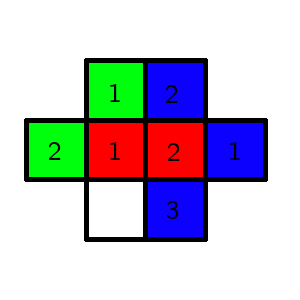
\includegraphics[scale=0.42,angle=0]{afsnit/vores_implementation/billeder/flood_fill/floodfill4}
    \end{center}
    \caption[]{Pixels efter skridt tre og et nyt skridt 1. Vi har valgt
    den grønne pixel, med det laveste tal, fra figur \ref{floodfill3} som
    ny startpixel. Nye pixels markeret med blåt mangler at blive
    kontrolleret.}
    \label{floodfill4}
\end{figure}

På denne måde itererer metoden sig igennem alle de pixels, som ligger
inden for en vis afvigelse fra startfarven. Metoden kan bruges på to
måder; enten kan man regne varianten fra den første startpixel ud, og
således kun have én startfarve, eller man kan ændre den efter den nye
startpixel --- som bliver fundet i tredje skridt --- og således have en
startfarve, der ændres efterhånden. Det skal bemærkes, at den pixel, som
i figur \ref{floodfill3} mister sit blå flag, godt kan blive taget i
betragtning igen senere, når vi vælger en ny startpixel. En pixel kan
dog højst blive taget i betragtning i alt fire gange, fordi den har fire
tilstødende pixels.

\subsubsection{Eksempler}
Vi vil nu eksemplificere, hvordan denne metode virker i praksis ved
manipulation af billedet vist i figur \ref{bathers}.  Dette billede er
valgt, da det har været brugt i flere argumenter for, at man i
malerkunsten finder særligt mange interessante regioner i det gyldne
snit\cite{GoldenNumber,RatioArt}. Endvidere er maleriet
interessant at teste på, da det er udført i det, der kaldes
pointilistisk stil, hvilket vil sige, at maleriet faktisk består af en
masse små prikker. I de fem billeder vist i figur
\ref{dot_ff_fixed_7_7}, \ref{dot_ff_var_7_7}, \ref{dot_ff_fixed_10_10},
\ref{dot_ff_var_10_10} og \ref{dot_ff_var_9_9} bruges floodfill på den
pixel, der er at finde i midten af den røde prik. Den tilladte afvigelse
gives som parret $(lo, up)$ med en værdi for, hvor meget RGB-værdien må
henholdsvis falde og stige. Det anbefales at studere figurene og den
tilhørende tekst.

% Det her billede opfører sig underligt mht. scale :/
\begin{figure}[!h]
    \begin{center}
        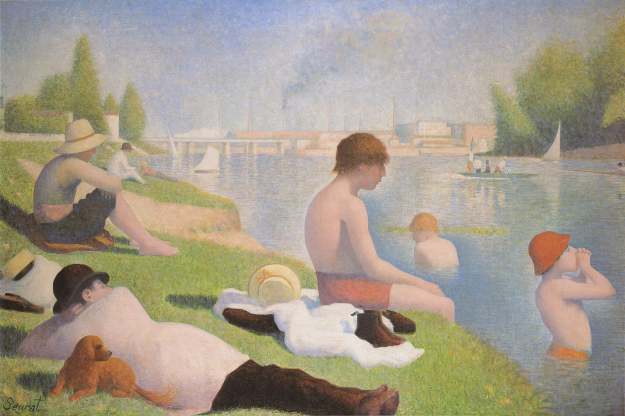
\includegraphics[scale=8]{afsnit/vores_implementation/billeder/flood_fill/seurat_bathers}
    \end{center}
    \caption[George Seurat: \emph{Bathers at Asnieres} -- 1884]{George
    Seurat: \emph{Bathers at Asnieres} - 1884\\Originalt billede.}
    \label{bathers}
\end{figure}

\begin{figure}[!h]
    \begin{center}
        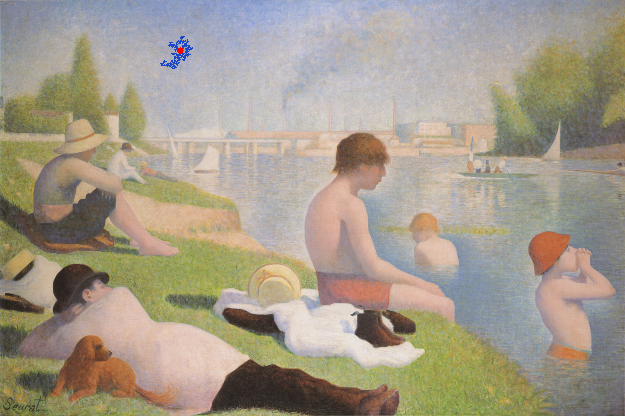
\includegraphics[scale=0.49]{afsnit/vores_implementation/billeder/flood_fill/dot_ff_fixed_7_7}
    \end{center}
    \caption[]{Floodfill-metoden i et billede, hvor der kun sammenlignes
    med farven på den originale pixel med afvigelsen $(7,7)$.}
    \label{dot_ff_fixed_7_7}
\end{figure}

\begin{figure}[!h]
    \begin{center}
        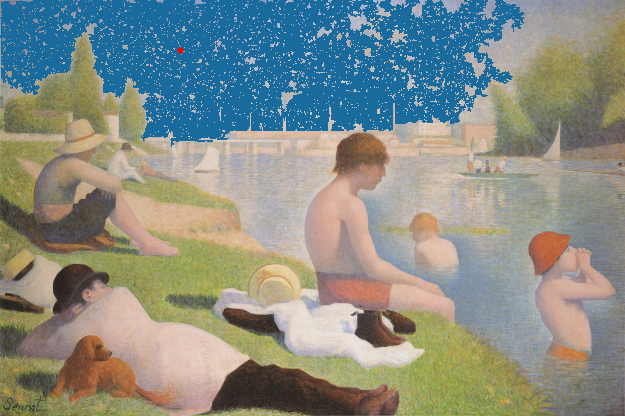
\includegraphics[scale=0.49]{afsnit/vores_implementation/billeder/flood_fill/dot_ff_var_7_7}
    \end{center}
    \caption[]{Floodfill-metoden i et billede, hvor der sammenlignes med
    farven på den nye startpixel. Afvigelsen er sat til $(7,7)$ ligesom
    i figur \ref{dot_ff_fixed_7_7}. Det ses, at vi nu dækker et meget
    større areal.}
    \label{dot_ff_var_7_7}
\end{figure}

\begin{figure}[!h]
    \begin{center}
        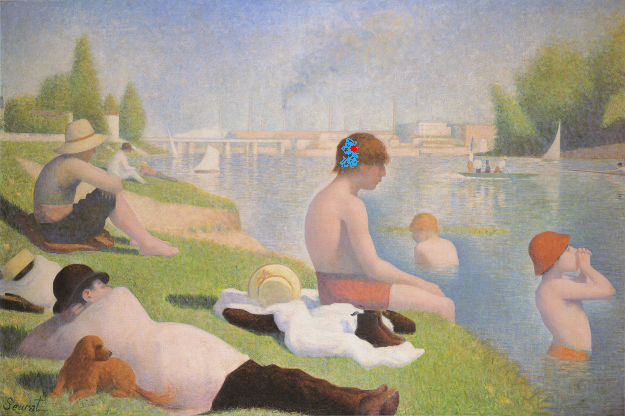
\includegraphics[scale=0.49]{afsnit/vores_implementation/billeder/flood_fill/dot_ff_fixed_10_10}
    \end{center}
    \caption[]{Floodfill-metoden i et billede, med udgangspunkt i en ny
    pixel, hvor der kun sammenlignes med den originale pixel. Den
    tilladte afvigelse er på $(10,10)$.}
    \label{dot_ff_fixed_10_10}
\end{figure}

\begin{figure}[!h]
    \begin{center}
        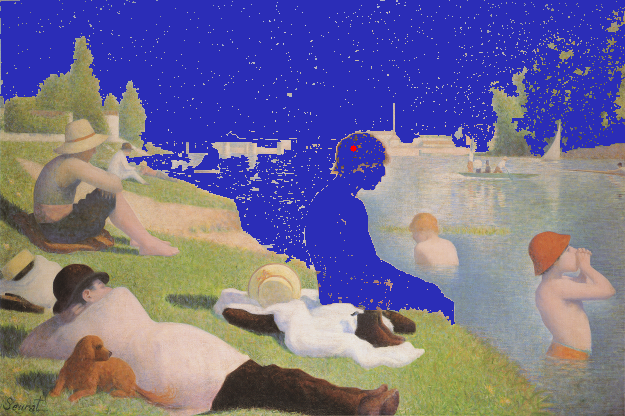
\includegraphics[scale=0.49]{afsnit/vores_implementation/billeder/flood_fill/dot_ff_var_10_10}
    \end{center}
    \caption[]{Floodfill med samme udgangspunkt og afvigelse som i figur
    \ref{dot_ff_fixed_10_10}, men der sammenlignes nu med den nye
    startpixel. Med en større tilladt afvigelse, breder floodfill sig
    meget mere og smelter både himmel, hav og dreng sammen.}
    \label{dot_ff_var_10_10}
\end{figure}

\begin{figure}[!h]
    \begin{center}
        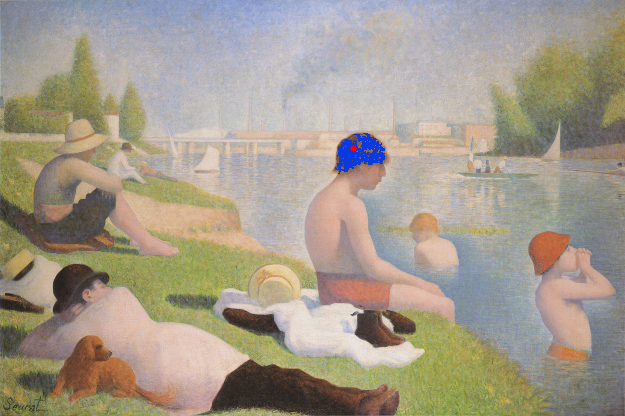
\includegraphics[scale=0.49]{afsnit/vores_implementation/billeder/flood_fill/dot_ff_var_9_9}
    \end{center}
    \caption[]{Floodfill med samme udgangspunkt som i figur
    \ref{dot_ff_fixed_10_10} og \ref{dot_ff_var_10_10}. Her bruges igen
    sammenligning med ny startpixel, men nu med en afvigelse på $9,9$.
    Denne lille ændring er nok til, at vi holder os pænt indenfor den
    region som udgøres af drengens hår.}
    \label{dot_ff_var_9_9}
\end{figure}

\subsubsection{Hvilken metode passer bedst?}
Som nævnt ovenfor, og illustreret i billederne, er der to måder vi kan
bruge floodfill på. Hvis man vælger at regne varianten ud fra den første
startpixel, ses det, at metoden vil indskrænke sig meget og ikke komme
ind i alle hjørner af en region. Til gengæld har denne fremgangsmåde
sværere ved at krydse kanter og på den måde komme ind i en ny region.

Vælger man at ændre varianten efter den nye startpixel, ses det, at man
vil male større regioner. Da denne fremgangsmåde hele tiden tilpasser
varianten, kan man medtage regioner, der langsomt skifter farve. Et godt
eksempel ses i figur \ref{dot_ff_var_10_10}, hvor drengens krop og
bukser bliver set som sammenhængende. Dette er interessant, især med
hensyn til digitale billeder af malerier, da solen eller blitzens
refleksion kan påvirke billedets farver. Af samme grund er den
fremgangsmåde heller ikke særlig følsom over for kanter, hvilket
resulterer i, at man let kommer til at gå ind i andre regioner.

Vi har valgt at benytte os af den sidstnævnte metode, da den efter vores
mening giver det bedste resultat. Vi vurderer, at det er vigtigere at
tage højde for sol og små farveskift end at være sikker på, at vi ikke
går ud over kanterne. Vi vil senere beskrive, hvordan vi på anden vis
sikrer, at vi beholder kanterne.

Som illustreret i billederne skal vi dog stadig tage højde for, hvordan
vi vil sætte tærskelværdierne. Indtil videre bliver de sat efter, hvad
der giver det mest illustrative resultat.

%For at få denne metode til at virke på 25000 billeder, hvor en del af
%billederne ikke har samme farvetone eller er blevet falmet, må der
%for hvert billede udregnes hvad for en varians i farve der skal bruges.

}

% vim: set tw=72 spell spelllang=da:


\subsection{Naiv algoritme}
{
% Image scale
\def\imgscale{0.34}

\textsf{Vi vil i det følgende forklare vores tanker bag en meget simpelt
fremgangsmåde, som har til formål at afgøre om et billede opfylder det
gyldne snit.  For at afgøre dette, trækker vi regioner ud af billedet og
vurderer dem efter deres placering, størrelse og form.  Vi siger at et
billede opfylder det gyldne snit, hvis en eller flere interessante
regioner kan siges at ligge i det gyldne snit.  I det følgende vil vi se
på hvornår en region ligger i det gyldne snit samt hvornår vi har med en
interessant region at gøre.
}

\subsubsection{Regionens placering}
Når vi har trukket regioner ud af et billede og vil afgøre om de ligger
i det gyldne snit, er det indlysende at deres placering har afgørende
betydning.  Vi vil nu komme frem til en definition hvorved man kan
afgøre om en region i billedet er placeret i det gyldne snit.

Vi starter med at se på det meget simple tilfælde, hvor en region
åbenlyst ligger placeret i det gyldne snit.  Et sådan eksempel ses i
figur \ref{pos_naiv_1}, hvor regionen vi betragter er farvet sort.  Den
røde linje markerer det gyldne snit.  Dette farveskema vil være
gennemgående i det følgende.  Det ses at regionen nærmest tangerer
linjen.

\begin{figure}[h]
	\begin{center}
		
\includegraphics[scale=\imgscale,angle=0]{afsnit/vores_implementation/billeder/naiv_algoritme/naiv_positiv_blob_1}
	\end{center}
	\caption[En positiv region]{En region som tangerer det gyldne snit.
	Denne region er positiv.}
	\label{pos_naiv_1}
\end{figure}

I praksis vil vi dog sjældent have at regioner ligger helt præcist på
snittet.  På grund af den måde, vi trækker regioner ud af billedet på,
kan vi ikke være sikre på at regionen er fyldt helt ud til dens kanter,
fordi der i disse områder stadig er stor overgang i farverne.  Dette
bevirker at en regioner kan blive repræsenteret som mindre end de
virkelig er.  Vi har også, at det gyldne snit baserer sig på det
irrationelle tal $\varphi$ og vi kan derfor ikke regne os helt nøjagtig
frem til vores det egentlige snit ligger.  Vi indfører derfor en margen
hvori vi vil acceptere regioner.  I praksis betyder det at vi ikke
\emph{kun} kigger på den linje der deler billedet ved det gyldne snit,
men faktisk tager vi et bånd, sammensat af en række snit, og bruger
dette bånd som et bredere gyldent snit.  Derved behøver en region ikke
at tangere det gyldne snit helt nøjagtig for at kunne betragtes som en
interessant region. F.eks. vil regionen i figur \ref{pos_naiv_margin_1}
anses som værende placeret i det gyldne snit.  Vær opmærksom på at vores
bånd, rent visuelt i de følgende illustrationer, er stærkt overdrevet.
\begin{figure}[h]
	\begin{center}
		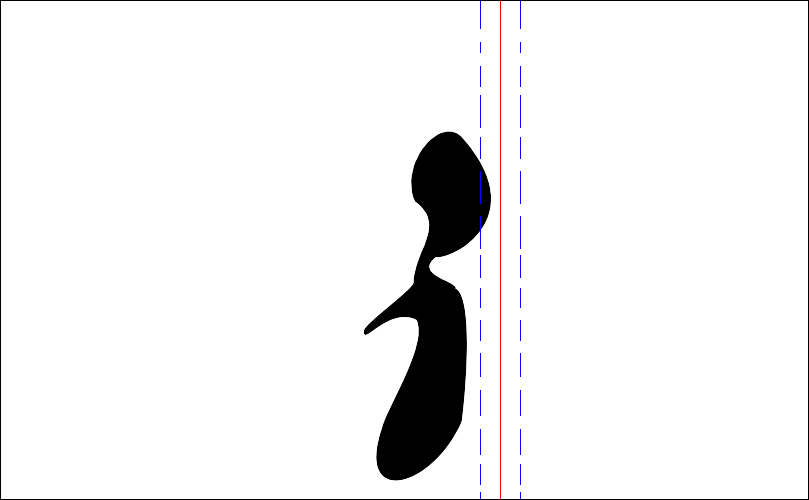
\includegraphics[scale=\imgscale,angle=0]{afsnit/vores_implementation/billeder/naiv_algoritme/naiv_positiv_blob_margin_1}
	\end{center}
	\caption[Positiv region i margen]{En region som
	ligger indenfor en margen af det gyldne snit betragtes som
	positiv. De blå stiplede linjer angiver vores bånd.}
	\label{pos_naiv_margin_1}
\end{figure}

Vi ser nu på det rektangel der der begrænser en region.  En side af
dette rektangel vil vi kalde for en kant.  Vi vil nu komme frem til, at
en region skal have mindst én kant indenfor båndet om det gyldne snit,
før vi kan sige at regionen ligger i det gyldne snit.

\begin{figure}[h]
	\begin{center}
		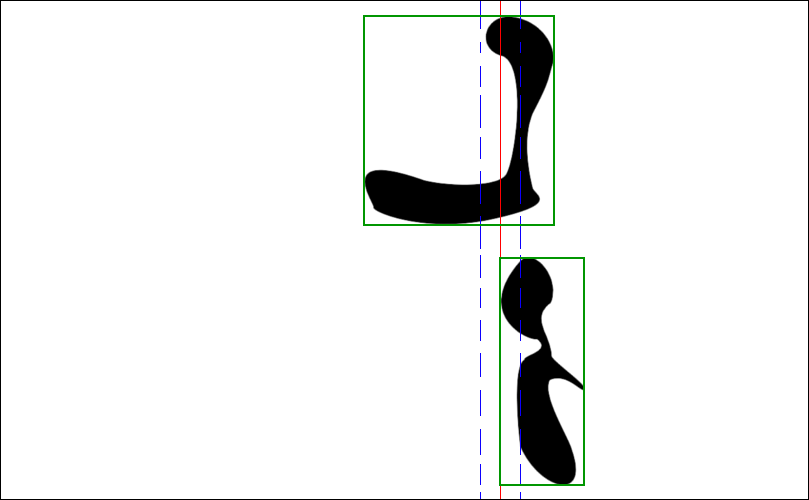
\includegraphics[scale=\imgscale,angle=0]{afsnit/vores_implementation/billeder/naiv_algoritme/bbox_section}
	\end{center}
	\caption[Afgrænsende rektangler]{Den øverste region kan ikke
	siges at ligge i det gyldne snit, da den ikke har nogen kanter
	indenfor båndet. Den nederste region derimod, har én kant
	indenfor båndet og ligger derfor i det gyldne snit.}
	\label{bbox_section}
\end{figure}

\begin{figure}[!h]
	\begin{center}
		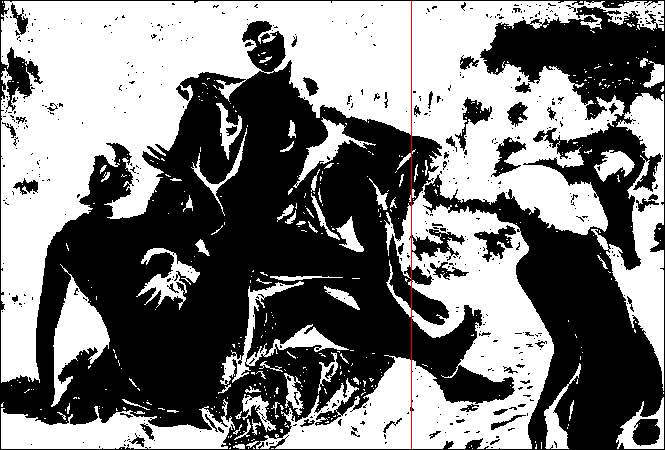
\includegraphics[scale=0.42,angle=0]{afsnit/vores_implementation/billeder/naiv_algoritme/bathers_mockup_blob}
	\end{center}
	\caption[Interessante regioner i praksis]{I praksis vil de
	fundne regioner være langt mere komplekse.}
	\label{realworld_example}
\end{figure}

Med denne definition på hvornår en region kan betragtes som liggende i
det gyldne snit, skal vi blot have en region med en kant indenfor vores
bånd.  I figur \ref{realworld_example} ses hvordan et rigtigt billede
kan tage sig ud når vi vil finde regioner.  Vi ser at der i dette
tilfælde vil blive udvalgt mange små regioner, som egentlig ikke kan
tillægges nogen betydning.  Vi vil nu gå videre og opsætte nogle
kriterier for hvornår en region er interessant.

\subsubsection{Regionens størrelse}
Når vi skal til at afgøre hvorvidt en region skal tages op til videre
overvejelse er det oplagt at se på størrelsen af regionen.  Vi siger
derfor at en region skal have en vis størrelse før den kan tages i
betragtning.  I praksis vil regionens areal afspejle dens størrelse,
hvor arealet er det antal pixels regionen optager i billedet.  Grænsen
for et acceptabelt areal skal sættes i forhold til billedets størrelse.

Omvendt er vi heller ikke interesseret i at få for store regioner med i
betragtningerne.  F.eks. vil en himmel i et maleri give en ret stor
sammehængende region.  De fleste af sådanne regioner vil dog ikke blive
taget i betragtning fordi de krydser snittet.  Hvis vi kigger på det
meget simple billede i figur \ref{pos_naiv_1} skal man også huske på at
der faktisk vises to regioner. Den sorte skikkelse er en region ligesom
den hvide baggrund er en region.  Baggrunden kan ikke siges at være en
interessant region, hvorfor det er vigtigt at sortere disse regioner
fra.

Indtil videre har vi kun illustreret ét snit i billedet.  Der er
imidlertid tre andre snit hvor vi også kan dele et billede efter det
gyldne snit.  Hvor vi har kigget på et vertikalt snit, vender vi nu
opmærksomheden mod et horisontalt snit.  Det generelle tilfælde vil være
at en region kun er interessant i forhold til enten et vertikalt eller
et horisontalt snit.  Et eksempel på dette ses i figur
\ref{pos_horiz_naiv_margin_1}.  Der kan dog forekomme specialtilfælde,
hvor en region vil være positiv i flere snit, hvilket vi vil komme ind
på i et senere kapitel.
\begin{figure}[H]
	\begin{center}
		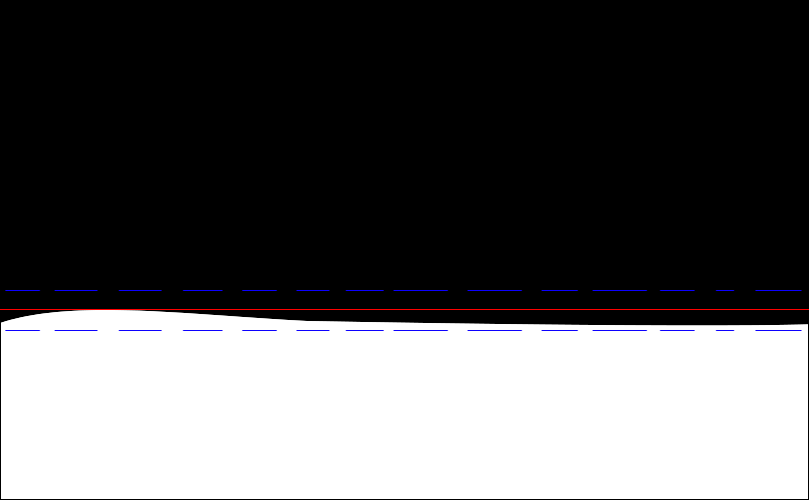
\includegraphics[scale=\imgscale,angle=0]{afsnit/vores_implementation/billeder/naiv_algoritme/naiv_horiz_positiv_blob_1}
	\end{center}
	\caption[Positiv horisontal region]{En positiv region med en
	kant i et horisontalt bånd.}
	\label{pos_horiz_naiv_margin_1}
\end{figure}
Det ses tydeligt at regionen i figur \ref{pos_horiz_naiv_margin_1} ikke
kan tages i betragtning i forhold til et vertikalt snit, da regionen,
uanset snittets placering, vil krydse dette.  Det ses dog at regionen
har en kant indeni et horisontalt bånd og derfor kan klassificeres som
en region der ligger i det gyldne snit.

\subsubsection{Regionens form}
Regionens form kan give informationer om hvorvidt vi har med en
interessant region at gøre.  I praksis er det dog meget svært at sige
noget om selve den fysiske form af en region, men vi kan sige noget om
dens masse.  En regions masse skal forstås som forholdet mellem
regionens areal og arealet af det rektangel der afgrænser regionen.
Dette forhold giver information om hvor massiv en region er.  En massiv
region vil være mere interessant end en meget spinkel region.  Figur
\ref{region_mass} illustrerer to forskellige regioner med forskellig
masse.
\begin{figure}[h]
	\begin{center}
		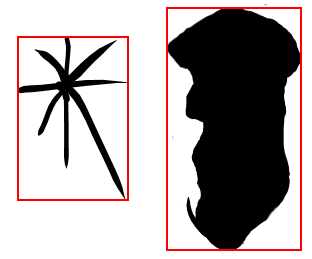
\includegraphics[scale=\imgscale,angle=0]{afsnit/vores_implementation/billeder/naiv_algoritme/bbox_area_ratio}
	\end{center}
	\caption[Regioners masse]{To forskellige regioner med vidt forskellige forhold
	mellem selve regionens areal og arealet af det rektangel der
	afgrænser regionen.}
	\label{region_mass}
\end{figure}
I praksis vil der blive udregnet et tærskel i forhold til et billedes
størrelse for hvor massiv en region skal være for at kunne
karakteriseres som interessant.

\subsubsection{Sammenfatning af betingelser}
Vi samler nu op på de ovenstående krav for bestemmelse af en interessant
region liggende i det gyldne snit.

\noindent For at en region kan betegnes som interessant og liggende i
det gyldne snit skal den
\begin{enumerate}
	\renewcommand{\labelenumi}{(\alph{enumi})}
	\item have en kant i båndet om det gyldne snit
\end{enumerate}
og regionen må
\begin{enumerate}
	\renewcommand{\labelenumi}{(\alph{enumi})}
	\setcounter{enumi}{1}
	\item \textbf{ikke} krydse båndet der deler billedet ved det gyldne snit;
	\item \textbf{ikke} have et areal mindre end en variabel tærskel der sættes i
		forhold til billedets størrelse
	\item \textbf{ikke} have en masse mindre end variabel tærskel.
\end{enumerate}
Vi har allerede argumenteret for at hvis betingelse $(a)$ er opfyldt
følger det trivielt at betingelse $(b)$ også er opfyldt.  Vi kan da
udlede, at hvis $(a)$ er opfyldt skal vi blot kontrollere $(c)$ og
$(d)$.  Når regionerne i nærheden af det gyldne snit er trukket ud af
billedet er det ligetil at kontrollere betingelserne$(a)$, $(c)$ og
$(d)$ ud fra deres begrænsende rektangel.

Et billede opfylder altså det gyldne snit hvis vi har en eller flere
interessante regioner der ligger i det gyldne snit.  Det er oplagt at
give regioner som er positiv i flere snit større vægt, hvilket vi også
vil komme ind på i et senere kapitel.

\subsubsection{Begrænsninger}
Denne naive tilgang har nogle begrænsninger.  Den mest åbenlyse er, at
regioner med symmetriakse i det gyldne snit, men med kanter udenfor
båndet ikke vil blive karakterisseret som liggende i det gyldne snit.
Regioner hvor et segment af denne faktisk ligger i båndet, som den
øverste region i figur \ref{bbox_section} hvor den vertikale del faktisk
ligger i snitter, vil ikke blive udvalgt.  Det kræver en videre
segmentering af de fundne regioner før at sådanne regioner vil blive
udvalgt.

}

% vim: set tw=72 spell spelllang=da:


\subsection{Opbevaring af resultater\label{section_results}}
{
Når vi har trukket regioner ud af billedet og vurderet dem efter
ovenstående simple algoritme kan vi stå tilbage med et egentligt
resultat. Vi ønsker at gemme dette resultat i en database så vi på et
senere tidspunkt kan bruge det i en samlet analyse af resultaterne.
Vi så i afsnit \ref{section_opbv_billeder} på et databaseskema til
opbevaring af maleriers metadata. Vi bygger nu videre på dette skema så
vi kan tilknytte resultater fra en analyse til de enkelte malerier. Det
fulde databaseskema ses nedenfor.

\begin{table}[!h]
    \centering
    \begin{tabular}{|l||c|c|c|c|c|c|}
        \hline
        \bf{artist} \hspace{0.5cm} & \underline{artistId} & name & born & died & school & timeline \\\hline
    \end{tabular}
    \caption{Databasetabel for kunstner}
    \label{artistTable}
\end{table}

\begin{table}[!h]
    \centering
    \begin{tabular}{|l||c|c|c|c|c|c}
        \hline
        \bf{painting} \hspace{0.5cm} & \underline{paintingId} & artistId & title & date & paint & $\cdots$ \\\hline
    \end{tabular}\\ \vspace{0.2cm}\hspace{1.2cm}
    \begin{tabular}{c|c|c|c|c|c|c}
        \hline
        $\cdots$ & material & location & url & form & type & $\cdots$ \\\hline
    \end{tabular}\\ \vspace{0.2cm}\hspace{1.4cm}
    \begin{tabular}{c|c|c|c|c|c|}
        \hline
        $\cdots$ & realHeight & realWidth & height & width & filepath \\\hline
    \end{tabular}
    \caption{Databasetabel for malerier}
    \label{paintingTable}
\end{table}

\begin{table}[!h]
    \centering
    \begin{tabular}{|l||c|c|c|c|c|c|c|}
        \hline
        \bf{run} \hspace{0.5cm} & \underline{runId} & trsh1 & trsh2 & lo & up & marginPercentage & method \\\hline
    \end{tabular}
    \caption{Databasetabel for en kørsel}
    \label{runTable}
\end{table}

\begin{table}[!h]
    \centering
    \begin{tabular}{|l||c|c|c|c|c|c|}
        \hline
        \bf{result} \hspace{0.5cm} & \underline{resultId} & runId & paintingId & cutRatio & cutNo & numberOfRegions \\\hline
    \end{tabular}
    \caption{Databasetabel for resultater}
    \label{resultTable}
\end{table}

\begin{table}[!h]
    \centering
    \begin{tabular}{|l||c|c|c|c|c|c|c|}
        \hline
        \bf{region} \hspace{0.5cm} & \underline{regionId} & resultId & x & y & height & width & area \\\hline
    \end{tabular}
    \caption{Databasetabel for regioner}
    \label{regionTable}
\end{table}

Tabellerne \ref{artistTable} og \ref{paintingTable} er de samme som vist
i afsnit \ref{section_opbv_billeder}, men er taget med her blot for at
vise databaseskemaet i sin helhed. Det øvrige databaseskema lægger vægt
på at minimere redundans og mulighed for at genskabe kørte analyser.
Sidstnævnte er vigtig osv\dots

}
% vim: set tw=72 spell spelllang=da:


}

% vim: set tw=72 spell spelllang=da:
